\section{Lebenslauf}
\newpage

\section{Management Summary}
Themenbeschreibung\\
Entwicklung einer Open-Source Projektmanagement-Applikation für Videospiel-Einzelentwickler und
kleine Entwicklerteams welche mit Unity3D arbeiten. Dabei sollen die Wichtigsten Funktionen direkt
in Unity selber verfügbar sein
Kunde
Potenzielle Kunden sind alle Einzelentwickler / Entwicklerteams, welche mit Unity3D arbeiten
Erfolgskriterien
- Eine WPF-Applikation wurde den Anforderungen (siehe: Ziele und Anforderungen)
entsprechend entwickelt.
- Ein in Unity integriertes Benutzerinterface (Custom Editor) in welchem Aktivitäten zum
aktuellen Projekt angesehen/bearbeitet werden können wurde den Anforderungen (siehe:
Ziele und Anforderungen) entsprechend entwickelt.
- Es Liegt eine vollständige Dokumentation des Projektes vor
- Die Applikation ist als Open-Source Software lizensiert und zum Download verfügbar

\newpage

\section{Initialisierung}
\newpage


\subsection{Planung}

Es wird mit einer abgewandelten Form des Wasserfallmodells geplant.
Dabei wird das Projekt in 5 Phasen aufgeteilt: \\
\begin{enumerate}
  \item Initialisierung
  \item Analyse
  \item Konzept
  \item Umsetzung / Realisierung
  \item Veröffentlichung
\end{enumerate}
\vspace{1cm}
In den einzelnen Phasen werden Tasks geplant, welche eine geschätzte Dauer zur umsetzung haben.
Anhand dieser Schätzung wird die Dauer der einzelnen Phasen geplant. Zusätzlich wird pro Phase ein Buffer eingeplant.
\vspace{0.5cm}\\
Um das Projekt zu planen habe ich mir zuerst die einzelnen Phasen in einer Gantt-Diagramm-form ausgelegt.
Anschliessend bin ich Phase für Phase durchgegangen un habe mir Tasks erstellt, anhand der Schäzung der Dauer habe ich überprüft,
ob die Phasenaufteilung passt.\\
Die Tasks sind in anzahl Tagen geplant, die länge der Tasks ist jedoch auch von meinem Zeitkontingent an den entsprechenden Tagen abhängig,
so kann z.B. ein 6h Task 3 Tage andauern, da ich nur 2h pro Tag verplanen konnte.
in der Woche vom 17.10.2022 habe ich eine Intensiv Woche geplant. In dieser Woche habe ich die Möglichkeit vollzeit an der Diplomarbeit zu arbeiten.
Daher ist in dieser Woche auch der Hauptteil der Umsetzung geplant.\\
Nach dem ich mir die Gantt-Diagramme gemacht und die einzelenen Tasks tabellarisch aufgelistet habe. 
Habe ich mir in einer Zeit-Tracking App (Toggle) alle Tasks angelegt. In Toggle erfasse ich somit die geleistete Arbeitszeit zu jeweiligem Task.\\
Dies soll mir ermöglichen verzögerungen schnell erkennen zu können und entsprechende Massnahmen einzuleiten.\\
Zum Controlling notiere ich mir die effektiv benötigte Zeit pro Task und kann somit das Zeitdelta berechnen.
\newpage
\subsubsection{Grobplanung}
Um die Planung etwas übersichtlicher zu gestalten, hab ich eine Grobplanung mit den einzelnen Phansen erstellt\\
Jede Phase wird in den folgenden Abschnitten noch detailierter geplant.
\begin{figure}[H]
    \begin{center}
      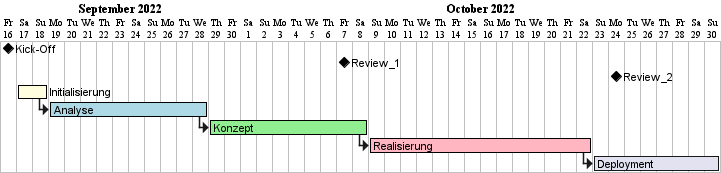
\includegraphics[width=1\linewidth]{../content/diagrams/gantt/roughtPlanning/roughtPlanning.png}
      \caption{GANTT Grobplanung}
    \end{center}
  \end{figure}
  \subsubsection{Initialisierung}
  \begin{figure}[H]
    \begin{center}
      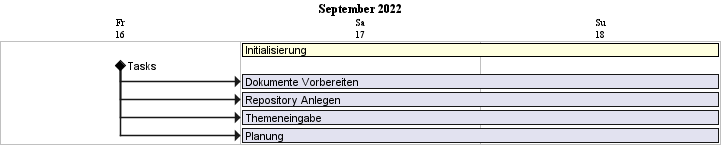
\includegraphics[width=1\linewidth]{../content/diagrams/gantt/InitializationPlanning/initializationPlanning.png}
      \caption{GANTT Initialisierung}
    \end{center}
  \end{figure}
  \begin{table}[H]
    \centering
    \settowidth\tymin{executeIncomingCommand()}
    \setlength\extrarowheight{2pt}
    \begin{tabulary}{1.0\textwidth}{|L|L|L|L|L|}
      \hline
      \textbf{Task} &
      \textbf{Beschreibung} &
      \textbf{Geplant}&
      \textbf{Ist}&
      \textbf{Delta}\\
      \hline
      Dokumente Vorbereiten &
      LaTex-Dokument aufsetzten, PlantUML Diagrammvorlagen erstellen &
      4h &
      3h&
      -1h\\
      \hline
      Repository Anlegen &
      GitHub Repos für Dokumentation und Projekt anlegen &
      1h &
      1h&
      0h\\
      \hline
      Themeneingabe &
      Themeneingabe in Dokumentation einfügen &
      1h &
      0.5h&
      -0.5h\\
      \hline
      Planung &
      Projektplanung Durchführen &
      6h &
      3.5h&
      -2.5\\
      \hline
      \textbf{Total} &
       &
      \textbf{12h} &
      \textbf{8h}&
      \textbf{-4h}\\
      \hline 
    \end{tabulary} 
    \caption{Initialisierungs Tasks}
  \end{table}

  \subsubsection{Analyse}
  \begin{figure}[H]
    \begin{center}
      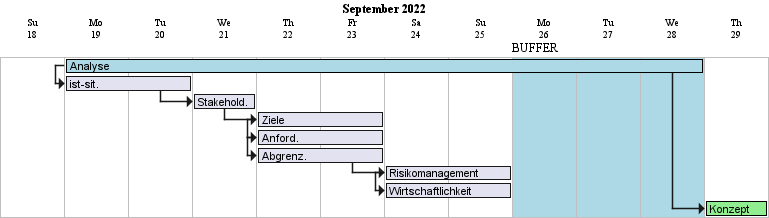
\includegraphics[width=1\linewidth]{../content/diagrams/gantt/analisisPlanning/analisisPlanning.png}
      \caption{GANTT Analyse}
    \end{center}
  \end{figure}
  \begin{table}[H]
    \centering
    \settowidth\tymin{executeIncomingCommand()}
    \setlength\extrarowheight{2pt}
    \begin{tabulary}{1.0\textwidth}{|L|L|L|L|L|}
      \hline
      \textbf{Task} &
      \textbf{Beschreibung} &
      \textbf{Geplant}&
      \textbf{Ist}&
      \textbf{Delta}\\
      \hline
      Ist-Situation &
      Ausgangslage analysieren &
      4h &
      3h &
      -1h\\
      \hline
      Stakeholderanalyse &
      Stakeholder erfassen und gewichten &
      3h &
      2h &
      -1h\\
      \hline
      Ziele &
      Zielsetzungen aus Themeneingabe präzisieren &
      2h &
      3h &
      +1h\\
      \hline
      Anforderungen &
      Anforderungen aus Themeneingabe präzisieren &
      2h &
      1h &
      -1h\\
      \hline
      Abgrenzung &
      Abgrenzungen der Lösung definieren &
      3h &
      1h &
      -2h\\
      \hline
      Risikoanalyse &
      Risiken identifizieren und Massnahmen definieren &
      6h &
      2h &
      -4h\\
      \hline
      Wirtschaflichkeitsanalyse &
      Wirtschaflichkeit der Lösung eruiren &
      4h &
      1h &
      -3h\\
      \hline
      \textbf{Total} &
       &
      \textbf{24h} &
      \textbf{13h} &
      \textbf{-11h} \\
      \hline
    \end{tabulary}
    \caption{Analyse Tasks}
  \end{table}

  
  \subsubsection{Konzept}
  \begin{figure}[H]
    \begin{center}
      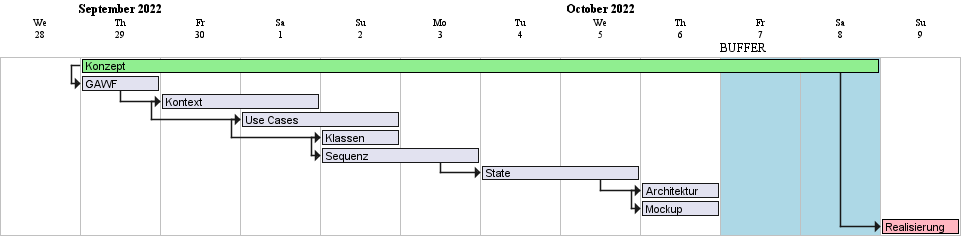
\includegraphics[width=1\linewidth]{../content/diagrams/gantt/conceptPlanning/roughtPlanning.png}
      \caption{GANTT Konzept }
    \end{center}
  \end{figure}
  \begin{table}[H]
    \centering
    \settowidth\tymin{executeIncomingCommand()}
    \setlength\extrarowheight{2pt}
    \begin{tabulary}{1.0\textwidth}{|L|L|L|L|L|}
      \hline
      \textbf{Task} &
      \textbf{Beschreibung} &
      \textbf{Geplant}&
      \textbf{Ist}&
      \textbf{Delta}\\
      \hline
      GAWF &
      Geschäftsanwendungsfälle beschreiben &
      6h &
      0h &
      \\
      \hline
      Kontext &
      Kontextdiagramm erstellen &
      3h &
      0h &
      \\
      \hline
      Use Cases &
      Use-Case-Diagramme erstellen&
      5h &
      0h &
      \\
      \hline
      Klassen &
      Klassendiagramm erstellen &
      2h &
      0h &
      \\
      \hline
      Sequenz &
      Sequenzdiagramme erstellen &
      4h &
      0h &
      \\
      \hline
      State &
      Statediagramme erstellen &
      3h &
      0h &
      \\
      \hline
      Test &
      Testkonzept erstellen &
      4h &
      0h &
      \\
      \hline
      Architektur &
      Planung der Software Architektur &
      3h &
      0h &
      \\
      \hline
      Mockup&
      Mockup der Applikationen erstellen &
      5h &
      0h &
      \\
      \hline
      \textbf{Total} &
       &
      \textbf{35h} &
      \textbf{0h}&
      \textbf{0h} \\
      \hline
    \end{tabulary}
    \caption{Konzept Tasks}
  \end{table}

  \subsubsection{Umsetzung}
  \begin{figure}[H]
    \begin{center}
      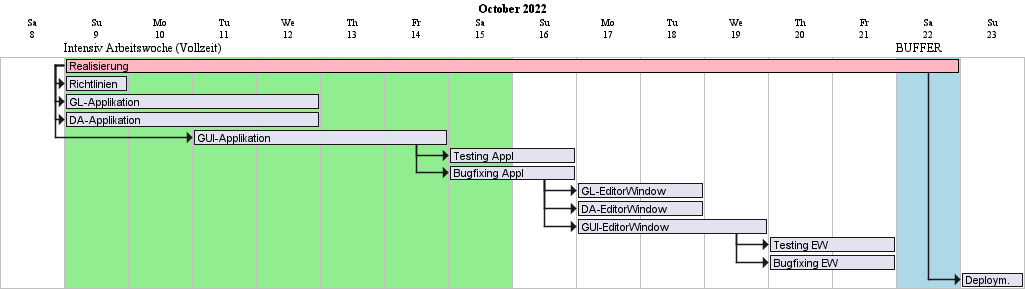
\includegraphics[width=1\linewidth]{../content/diagrams/gantt/realizationPlanning/realizationPlanning.png}
      \caption{GANTT Realisierung}
    \end{center}
  \end{figure}
  \begin{table}[H]
    \centering
    \settowidth\tymin{executeIncomingCommand()}
    \setlength\extrarowheight{2pt}
    \begin{tabulary}{1.0\textwidth}{|L|L|L|L|L|}
      \hline
      \textbf{Task} &
      \textbf{Beschreibung} &
      \textbf{Geplant}&
      \textbf{Ist}&
      \textbf{Delta}\\
      \hline
      Richtlinien &
      Coding Richtlinien definieren &
      2h &
      0h &
      \\
      \hline
      GL-Applikation &
      Geschäftslogik der Applikation implementieren &
      11h &
      0h &
      \\
      \hline
      DA-Applikation &
      Data handling der Applikation implementieren&
      6h &
      0h &
      \\
      \hline
      GUI-Applikation &
      GUI der Applikation implementieren &
      25h &
      0h &
      \\
      \hline
      Testing Applikation &
      Testen der Applikation anhand Testkonzept &
      6h &
      0h &
      \\
      \hline
      Bugfixing Applikation &
      Allfällige Bugs fixen / Buffer &
      8h &
      0h &
      \\
      \hline
      GL-EditorWindow &
      Geschäftslogik des EditorWindows implementieren &
      4h &
      0h &
      \\
      \hline
      DA-EditorWindow&
      Data handling des EditorWindows implementieren &
      4h &
      0h &
      \\
      \hline
      GUI-EditorWindow &
      GUI des EditorWindows implementieren &
      8h &
      0h &
      \\
      \hline
      Testing EditorWindow &
      Testen des EditorWindows anhand Testkonzept &
      4h &
      0h &
      \\
      \hline
      Bugfixing EditorWindow &
      Allfällige Bugs fixen / Buffer &
      6h &
      0h &
      \\
      \hline
      \textbf{Total} &
       &
      \textbf{84h} &
      \textbf{0h} &
      \textbf{0h} \\
      \hline
    \end{tabulary}
    \caption{Umsetzung Tasks}
  \end{table}

  \subsubsection{Deployment}
  \begin{figure}[H]
    \begin{center}
      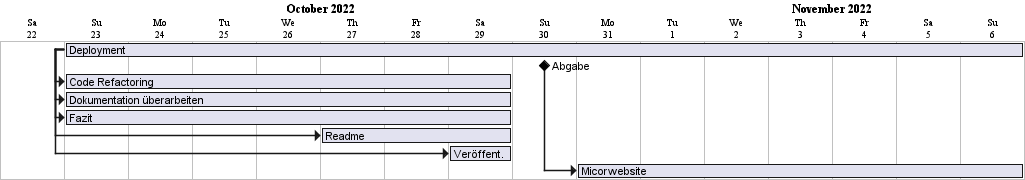
\includegraphics[width=1\linewidth]{../content/diagrams/gantt/deploymentPlanning/deploymentPlanning.png}
      \caption{GANTT Deployment }
    \end{center}
  \end{figure}
  \begin{table}[H]
    \centering
    \settowidth\tymin{executeIncomingCommand()}
    \setlength\extrarowheight{2pt}
    \begin{tabulary}{1.0\textwidth}{|L|L|L|L|L|}
      \hline
      \textbf{Task} &
      \textbf{Beschreibung} &
      \textbf{Geplant}&
      \textbf{Ist}&
      \textbf{Delta}\\
      \hline
      Code Refactoring &
      Code cleanup / Optimisierungen &
      5h &
      0h &
      \\
      \hline
      Dokumentation Überarbeiten &
      Fehlerkorrektur, Format &
      5h &
      0h &
      \\
      \hline
      Readme&
      Readme für GitHub-Page erstellen&
      3h &
      0h &
      \\
      \hline
      Veröffentlichen &
      GitHub Projekt veröffentlichen &
      2h &
      0h &
      \\
      \hline
      \textbf{Total} &
       &
      \textbf{15h} &
      \textbf{0h} &
      \textbf{0h} \\
      \hline
    \end{tabulary}
    \caption{Deployment Tasks}
  \end{table}



